\documentclass[a4paper,11pt]{article}
\usepackage{amsmath,amsthm,amsfonts,amssymb,amscd,amstext,vmargin,graphics,graphicx,tabularx,multicol} \usepackage[french]{babel}
\usepackage[utf8]{inputenc}  
\usepackage[T1]{fontenc} 
\usepackage[T1]{fontenc}
\usepackage{amsmath,amssymb}
\usepackage{pstricks-add,tikz,tkz-tab,variations}
\usepackage[autolanguage,np]{numprint} 

\setmarginsrb{1.5cm}{0.5cm}{1cm}{0.5cm}{0cm}{0cm}{0cm}{0cm} %Gauche, haut, droite, haut
\newcounter{numexo}
\newcommand{\exo}[1]{\stepcounter{numexo}\noindent{\bf Exercice~\thenumexo} : \marginpar{\hfill /#1}}
\reversemarginpar


\newcounter{enumtabi}
\newcounter{enumtaba}
\newcommand{\q}{\stepcounter{enumtabi} \theenumtabi.  }
\newcommand{\qa}{\stepcounter{enumtaba} (\alph{enumtaba}) }
\newcommand{\initq}{\setcounter{enumtabi}{0}}
\newcommand{\initqa}{\setcounter{enumtaba}{0}}

\newcommand{\be}{\begin{enumerate}}
\newcommand{\ee}{\end{enumerate}}
\newcommand{\bi}{\begin{itemize}}
\newcommand{\ei}{\end{itemize}}
\newcommand{\bp}{\begin{pspicture*}}
\newcommand{\ep}{\end{pspicture*}}
\newcommand{\bt}{\begin{tabular}}
\newcommand{\et}{\end{tabular}}
\renewcommand{\tabularxcolumn}[1]{>{\centering}m{#1}} %(colonne m{} centrée, au lieu de p par défault) 
\newcommand{\tnl}{\tabularnewline}

\newcommand{\trait}{\noindent \rule{\linewidth}{0.2mm}}
\newcommand{\hs}[1]{\hspace{#1}}
\newcommand{\vs}[1]{\vspace{#1}}

\newcommand{\N}{\mathbb{N}}
\newcommand{\Z}{\mathbb{Z}}
\newcommand{\R}{\mathbb{R}}
\newcommand{\C}{\mathbb{C}}
\newcommand{\Dcal}{\mathcal{D}}
\newcommand{\Ccal}{\mathcal{C}}
\newcommand{\mc}{\mathcal}

\newcommand{\vect}[1]{\overrightarrow{#1}}
\newcommand{\ds}{\displaystyle}
\newcommand{\eq}{\quad \Leftrightarrow \quad}
\newcommand{\vecti}{\vec{\imath}}
\newcommand{\vectj}{\vec{\jmath}}
\newcommand{\Oij}{(O;\vec{\imath}, \vec{\jmath})}
\newcommand{\OIJ}{(O;I,J)}

\newcommand{\bmul}[1]{\begin{multicols}{#1}}
\newcommand{\emul}{\end{multicols}}


\newcommand{\reponse}[1][1]{%
\multido{}{#1}{\makebox[\linewidth]{\rule[0pt]{0pt}{20pt}\dotfill}
}}

\newcommand{\titre}[5] 
% #1: titre #2: haut gauche #3: bas gauche #4: haut droite #5: bas droite
{
\noindent #2 \hfill #4 \\
#3 \hfill #5

\vspace{-1.6cm}

\begin{center}\rule{6cm}{0.5mm}\end{center}
\vspace{0.2cm}
\begin{center}{\large{\textbf{#1}}}\end{center}
\begin{center}\rule{6cm}{0.5mm}\end{center}
}



\begin{document}
\pagestyle{empty}
\titre{Interrogation : Calcul littéral}{Nom :}{Prénom :}{Classe}{Date}




\exo{2.5}  Simplifier chacune des écritures suivantes en supprimant les symboles "$\times$" et les parenthèses inutiles :
 
\bmul{2}
\begin{flushleft}
$12 \times a \times 5 \times b = ....................... $ \\
\end{flushleft}

\begin{flushleft}
$ 4 \times (6 \times
c +7) - (25\times b ) =  . . . . . . . . . . . . . . . . . . . . . . . . . . $
\end{flushleft}

\columnbreak

\begin{flushleft}
	$  z \times 9 \times z \times z + 5 \times c \times 8 \times c = .............................. $ \\
	\end{flushleft}	
	




\begin{flushleft}
        $ ( x \times 3 - 1,7) \times (t - 5)       = .............................. $ \\   
        \end{flushleft}        

\emul

\vspace*{0.75cm}

\exo{1} Exprimer la longueur AB en fonction de $x$ :\\

\includegraphics[scale=1.1]{cclitt1.eps} \\

\reponse[1]\\

\vspace*{0.75cm}


\exo{3} Calculer chacune des expressions suivantes pour a=7 et b=3 .

\bmul{2}

$ G =5b - a $  \\
\reponse[4]\\

$M =2a + b^{2} - 40 $\\
\reponse[4]\\

\columnbreak

$F = \dfrac{9b - a}{ab}$\\
\reponse[4]\\

$Z = (b+a)(10b-a) $\\
\reponse[4]\\

\emul


\vspace*{0.75cm}

\exo{1.5}  On donne l'égalité suivante : $x^{2} + y^{2}= 10x - 2y - 1$ .\\
 L'égalité est-elle vérifiée pour $x=9$ et $y= 2$ ?\\
 
\noindent \reponse[5]\\



\newpage

\vspace*{0.25cm}

\exo{2} La formule de Platon pour construire des triangles rectangles est la suivante :\\

" Pour tous $n$, les nombres entiers supérieurs à 1, le triangle ABC tel que :\\
 $AB = 2n$ \hspace*{0.2cm},\hspace*{0.2cm} $ AC = n^{2}-1$ \hspace*{0.2cm} et \hspace*{0.2cm} $ BC = n^{2} + 1$, 
est toujours un triangle rectangle."\\

\textbf{Faire les calculs pour n = 3, puis construire le triangle en vraie grandeur. Repérer l'angle droit avec l'équerre.}\\

\noindent \reponse[3]\\

\vspace*{6.5cm}



\exo{} Bonus

\bmul{2}

\begin{flushleft}
\includegraphics[scale=0.8]{perimlitteral.eps} 
\end{flushleft}

\columnbreak

\initq \q Exprimer le périmètre de ce polygone.\\
\reponse[2]\\

\q Exprimer l'aire de ce polygone.\\
\reponse[4]\\


 \emul

\q Pour quelle valeur de $x$ le périmètre de ce polygone est-il égal à 40 cm ?\\
\reponse[4]\\




\end{document}
